\chapter*{Discussion}
\label{ch:discussion}
The results presented in the previous chapter show general
uncertainty in the models. This has a few possible explanations:
one of the most likely is general overlapping of features. One of the most likely
explanations is the significant overlap of features.\\

There are signs that point to this in neural networks' performance representations,
especially recurrent architectures.
This is evident during training, where meaningful improvements on training are
observed only in later epochs, as shown in the training and validation accuracy
plots (figure [...]): as soon as training accuracy starts rising meaningfully,
the model tends to overfit. Some interesting information can also be seen in
the confusion matrix and the class-wise accuracy plot, where the general tendency
for each training is to get a predominant class with a large number of predictions,
and a second one with a large percentage of correct predictions, while the rest of
the classes is left behind with few predictions going their way.
The convolutional architecture does not have the same tendency (figure [...]):
training accuracy rises in earlier epochs, without meaningful results in validation
accuracy.
By applying a filter to exclude the most common words, it's possible that the
remaining words carry less ambiguous emotional meanings, and are easier to interpret.\\
% TODO quote figures

An interesting aspect of the explainability analysis is the visualization of the results.
The \textbf{left section} of the graph in Figure~\ref{fig:expl} displays the predicted probabilities for each class. In the \textbf{center section}
feature importances are ranked from most to least relevant and divided into two groups: on the right
features with a positive influence on the predicted label; on the left, those with a negative influence that suggest the model should consider other classes.
The \textbf{right section} of the graph highlights the values of the most important
features, using bright colors to indicate features with a positive influence on the prediction.

\begin{figure}[H]
    \centering
    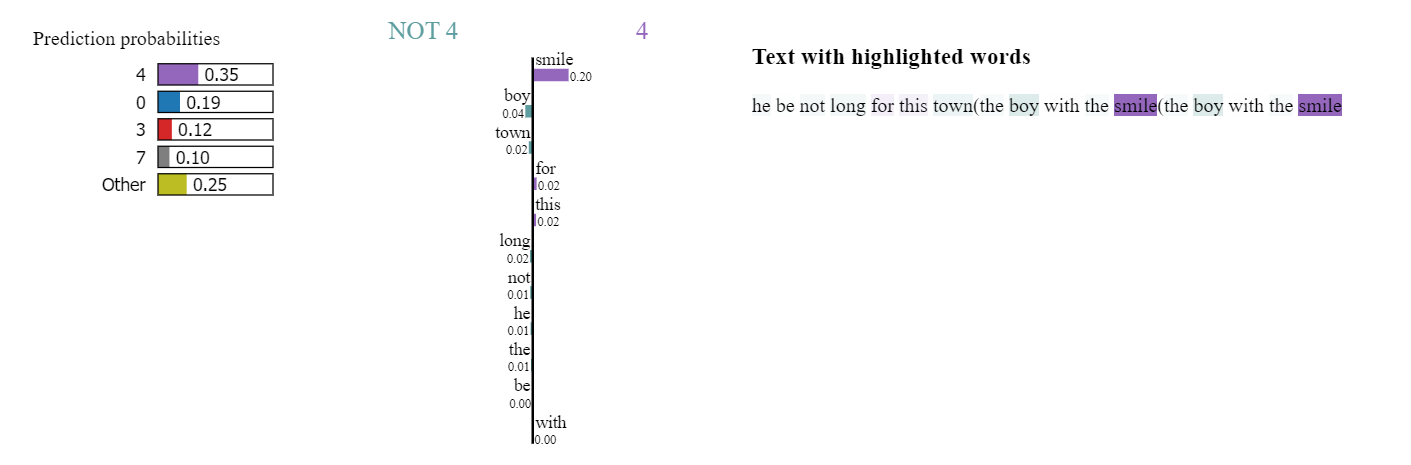
\includegraphics[scale= 0.55]{pictures/expl.png}
    \caption{Explainability - visualization}
    \label{fig:expl}
\end{figure}

The figure above illustrates a prediction where the model assigned the label \textit{joy} to the stanza under analysis, but the correct label, assigned by the ALBERT model (as mentioned in the \textit{Methods} section), was \textit{sadness}.
However, the word \textit{smile}, which is brighty highlighted, intuitively suggests that \textit{joy} might be a more plausible class for this stanza, even one that ALBERT could reasonably assign. 
This observation raises a critical issue: the transfer learning approach used to create the ground truth appears to have some limitations; in some instances the SVC model assigns a label that seems more contextually appropriate for the stanza, 
yet it differs from the supposedly correct label provided by ALBERT.\\

